
\documentclass{beamer}
\usepackage[T1]{fontenc}
\usepackage[french]{babel}
\usepackage[utf8]{inputenc}
\usepackage{amsmath}
\usepackage{amsfonts}
\usepackage{amssymb}
\usetheme{Warsaw}


\author[Adrien, Françoise, Julie, Luc, Nico*2, Thibaut, Vincent]{Adrien Leblond, Françoise Juvanon \\ Julie Le Callonnec, Luc Mazon \\ Nicolas Cattaneo, Nicolas Pellissier \\ Thibaut Lorrain, Vincent Durmont}
\title[Harbor Master]{Harbor Master}
\date{08 juin 2011}
% \logo{\includegraphics[scale=0.04]{/Images/logoPICSous.png}}

\addtobeamertemplate{footline}{\hfill\insertframenumber/\inserttotalframenumber\hspace{2em}\null}

\begin{document}
\begin{frame}<beamer>%Page de Présentation
  \titlepage
  ~\newline
  ~\newline
  ~\newline
  ~\newline
  ~\newline
  ~\newline
\end{frame}
% \begin{picture}(0,0)
%   \put(-38,0){\includegraphics[width=5cm]{commun/imagesCommunes/image}}
% \end{picture}

% \begin{picture}(0,0)
%   \put(100,30){\includegraphics[width=5cm]{image/PICSous_L_Ilogo.jpg}}
% \end{picture}



\begin{frame}[c]
  \tableofcontents%[hideallsubsections]
\end{frame}

%%%%%%%% 
%%%%%%%% INTRO ET PRESENTATION
%%%%%%%% 

\section{Présentation générale}
\begin{frame}[c]
  \tableofcontents[currentsection, hideothersubsections]
\end{frame}
\begin{frame}[c]
  \begin{block}{Contraintes}
\begin{description}
\item[Architecture distribuée]
~
  \begin{itemize}
  \item un serveur centralisant les données du jeu
  \item des clients pouvant interagir avec le jeu
  \item un client web permettant la simple visualisation de parties du jeu
  \end{itemize}
\item[Multi-utilisateur :] Plusieurs joueurs humains et/ou IA 
\item[Interfaces clientes génériques] possibilité de jouer avec divers périphériques d'entrée (souris, digitable \dots)
\item[Sauvegarde des parties] afin de pouvoir les revisionner par la suite
\end{description}

  \end{block}
\end{frame}



\section{Modèle}
\subsection{Éléments constitutifs}
\begin{frame}
\begin{block}{Eléments constitutifs du jeu}
  \begin{itemize}
  \item Jeu : Nombre de joueurs, Flotte, Score
  \item Bateau : Appartient à une flotte, type du bateau.
  \item Map : Carte du jeu, contient les ports.
  \end{itemize}
Permettent de modéliser un état de jeu, pas de le gérer.
  
\end{block}
\end{frame}

\subsection{Trajectoires et Collisions}
\subsection{Trajectoires}
 \begin{frame}[c]
\frametitle{Trajectoires}
   \begin{block}{Trajectoire}
     Une succession de directions
   \end{block}
  \begin{columns}
    \begin{column}[l]{5cm}
      \begin{figure}[!h]
        \begin{center}
          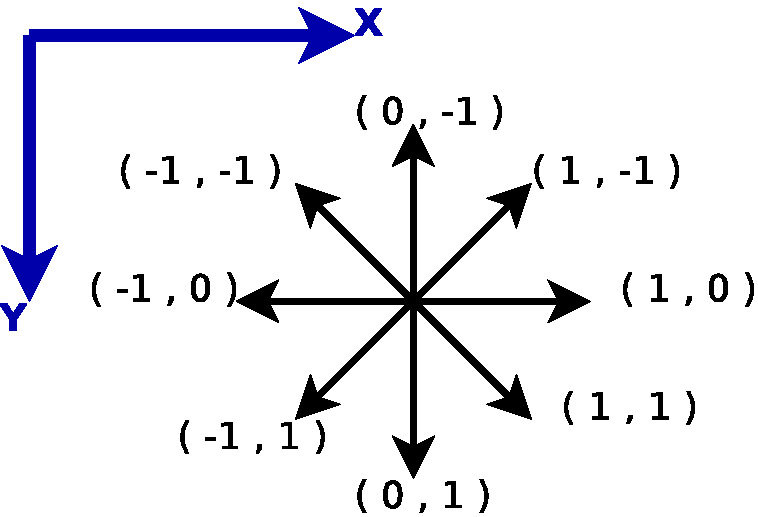
\includegraphics[scale=0.35]{./images/direction.pdf}
        \end{center}
        \caption{Direction}
      \end{figure}
    \end{column}
    \begin{column}[r]{5cm}
      \begin{figure}[!h]
        \begin{center}
          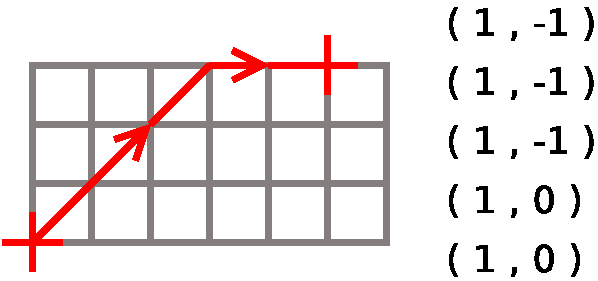
\includegraphics[scale=0.35]{./images/constructionTrajectoire.pdf}
        \end{center}
        \caption{Trajectoire}
      \end{figure}
    \end{column}
  \end{columns}
\end{frame}

\subsection{Collisions}
 \begin{frame}[c]
\frametitle{Collisions}
   \begin{block}{Objets à prendre en compte}
     \begin{itemize}
     \item Bateaux
     \item Berges de la carte
     \item Bords de la carte
     \end{itemize}
   \end{block}
         \begin{figure}[!h]
    \begin{center}
      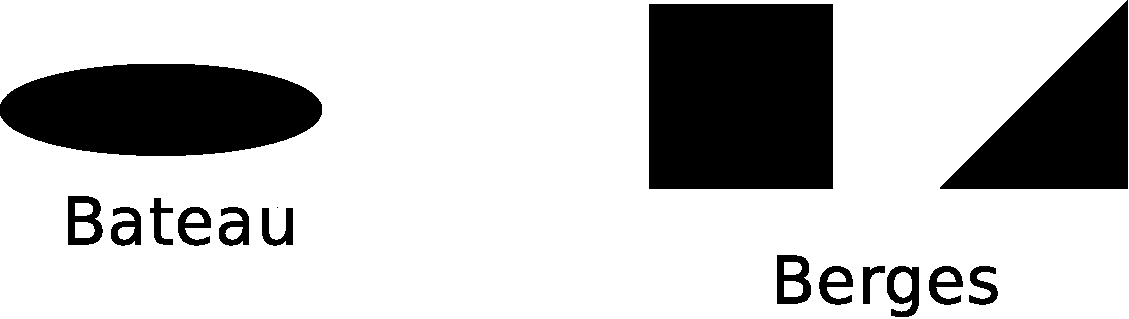
\includegraphics[scale=0.3]{./images/shape.pdf}
    \end{center}
    \caption{Les types de shape}
  \end{figure}
 \end{frame}


\section{Communication Client-Serveur}
\begin{frame}[c]
	\tableofcontents[currentsection, hideothersubsections]
\end{frame}

\subsection{Cahier des charges}
\begin{frame}[c]
	\frametitle{Cahier des Charges}
	\begin{block}{Besoins}
		\begin{description}
			\item[Client :] s'enregistrer, jouer, demander l'état du jeu, se désinscrire
			\item[Serveur :] envoyer un message à tous les utilisateurs
		\end{description}
	\end{block}
	\begin{block}{Contraintes}
		\begin{itemize}
			\item Réaliser une application distribuée avec un nombre illimité (?) de clients
			\item Clients de tous types : Linux, Android, iOS, Windows, Mac\dots{}
			\item Le jeu se déroule en temps réel et les actions d'un client influencent les autres clients
		\end{itemize}
	\end{block}
\end{frame}

\subsection{Technologies étudiées}
\begin{frame}[c]
	\frametitle{Technologies étudiées}
	\begin{block}{6 possibilités envisagées}
		\begin{itemize}
			\item Sockets
			\item RMI
			\item Corba
			\item WebServices
			\item EJB
			\item REST
		\end{itemize}
	\end{block}
\end{frame}

\begin{frame}[c]
	\frametitle{Sockets}
	\begin{block}{Avantages}
		\begin{itemize}
			\item Implémentation du minimum nécessaire : gain de rapidité
			\item Très bas niveau donc portable
		\end{itemize}
	\end{block}
	\begin{block}{Inconvénient}
		\begin{itemize}
			\item Difficulté de mise en place
		\end{itemize}
	\end{block}
\end{frame}

\begin{frame}[c]
	\frametitle{RMI}
	\begin{block}{Avantages}
		\begin{itemize}
			\item Callbacks inclus dans la technologie 
			\item Les objets sont situés côté serveur : gain de performance côté client
		\end{itemize}
	\end{block}
	\begin{block}{Inconvénient}
		\begin{itemize}
			\item Pas de librairie Android
		\end{itemize}
	\end{block}
\end{frame}

\begin{frame}[c]
	\frametitle{Corba}
	\begin{block}{Avantages}
		\begin{itemize}
			\item Callbacks inclus dans la technologie 
			\item Les objets sont situés côté serveur : gain de performance côté client
		\end{itemize}
	\end{block}
	\begin{block}{Inconvénients}
		\begin{itemize}
			\item Pas de librairie Android
			\item Difficulté de mise en place
		\end{itemize}
	\end{block}
\end{frame}

\begin{frame}[c]
	\frametitle{WebServices}
	\begin{block}{Avantages}
		\begin{itemize}
			\item Portabilité
			\item Simplicité de mise en place
		\end{itemize}
	\end{block}
	\begin{block}{Inconvénients}
		\begin{itemize}
			\item Callbacks absents sans un serveur (ex : JBOSS)
		\end{itemize}
	\end{block}
\end{frame}

\begin{frame}[c]
	\frametitle{EJB}
	\begin{block}{Avantages}
		\begin{itemize}
			\item Callbacks inclus dans la technologie 
		\end{itemize}
	\end{block}
	\begin{block}{Inconvénient}
		\begin{itemize}
			\item Pas de librairie Android
		\end{itemize}
	\end{block}
\end{frame}

\begin{frame}[c]
	\frametitle{REST}
	\begin{block}{Avantages}
		\begin{itemize}
			\item Architecture de haut niveau : simplicité d’implémentation
			\item Leger
			\item Framework complet dans Android et Java
			\item Framework compatible pour iOS (ASIHTTPRequest)
		\end{itemize}
	\end{block}
	\begin{block}{Inconvénients}
		\begin{itemize}
			\item Aucune connaissance préalable sur la vitesse de transfert
			\item Pas de callbacks
		\end{itemize}
	\end{block}
	\begin{center}
		$\Rightarrow$ notre choix s'est porté sur RESTLet !
	\end{center}
\end{frame}

\subsection{Architecture}
\begin{frame}[c]
	\frametitle{Architecture}
	\begin{center}
		\begin{figure}[h]
			\begin{center}
				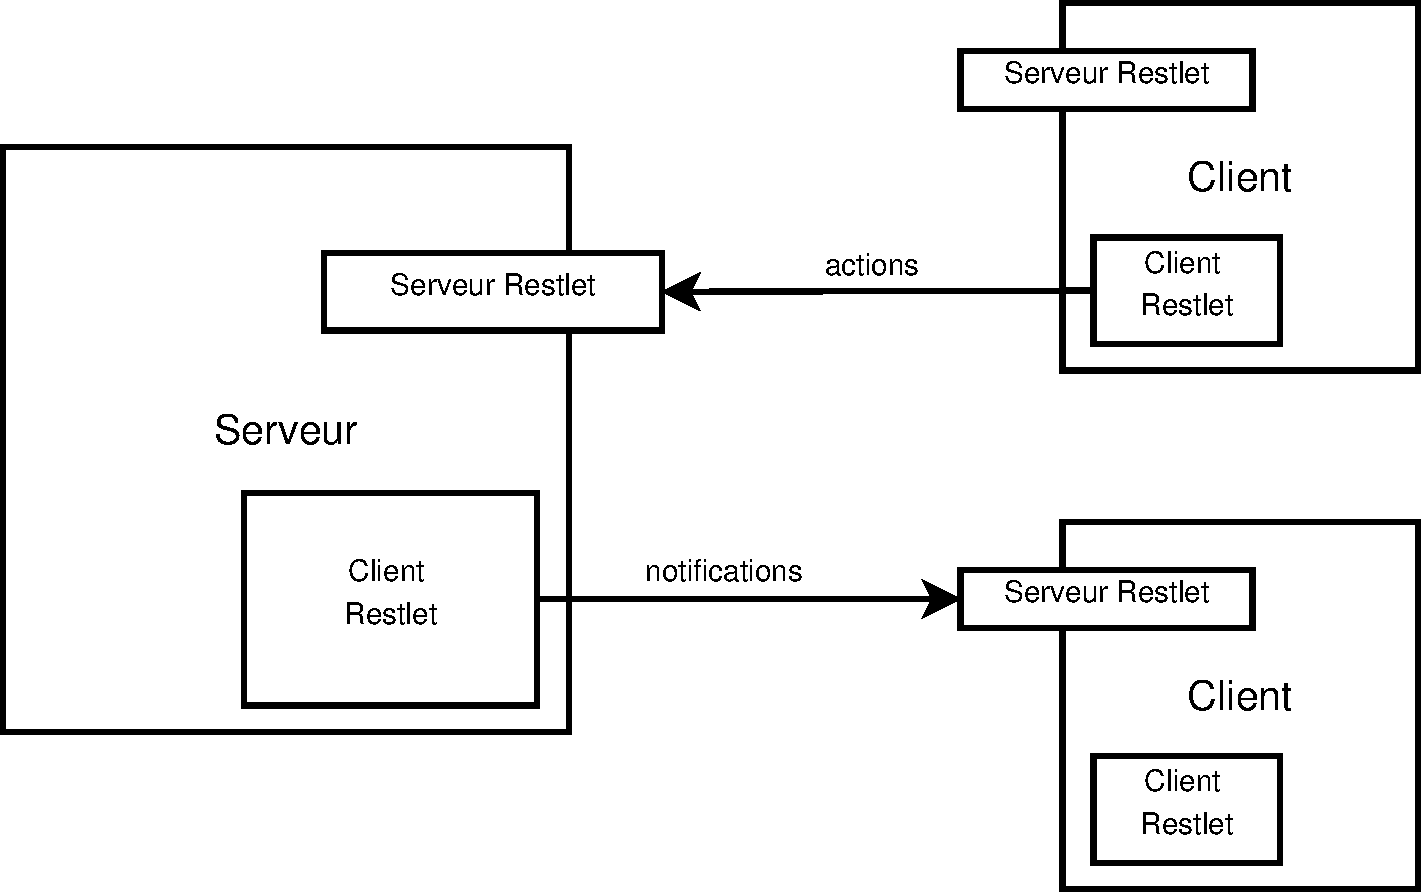
\includegraphics[width=0.8\textwidth]{images/communication}
			\end{center}
			\caption{Principe de communication en entre les clients et le serveur}
			\label{fig:comm}
		\end{figure}
	\end{center}
\end{frame}


\section{Interaction Client}
\begin{frame}[c]
\begin{block}{Contrainte}
Rappel du cahier de recette : l'interface client doit être générique. \\
\end{block}

\begin{block}{Classe Souris et interface EvenementClient}
\begin{description}
\item[interfaceEvenementClient] décrit les différentes fonctions qui permettent d'interagir avec le jeu (selectionnerBateau() \dots{})
\item[classe Souris] possède un attribut implémentant l'interface EvenementClient et appelle les fonctions de l'interface via ses propres fonctions (MousePressed \dots{}).
\end{description}
Il suffit de changer la classe Souris pour changer de périphérique d'entrée.
\end{block}
\end{frame}


\section{Affichage}
\begin{frame}[c]
  \tableofcontents[currentsection, hideothersubsections]
\end{frame}

\subsection{Slick}
\begin{frame}[c]
  \frametitle{Slick}
  \begin{block}{Caractéristiques}
    \begin{itemize}
    \item API de haut niveau java pour la conception de jeu en 2D;
    \item Basé sur l'API LWJGL librairie java reposant sur OpenGL.
    \end{itemize}
  \end{block}
  \begin{block}{Capacité de la librairie}
    \begin{itemize}
    \item Méthodes haut niveau pous la gestion d'un jeu;
    \item Gestion des images et des cartes facilités.
    \end{itemize}
  \end{block}
\end{frame}

\subsection{Map}
\begin{frame}[c]
  \frametitle{Tiled Map Editor}
  \begin{block}{Caractéristiques}
    \begin{itemize}
    \item Logiciel libre basé sur Qt (C++);
    \item Génération de cartes au format XML.
    \end{itemize}
  \end{block}
  \begin{block}{Utilisation dans notre cas}
    \begin{itemize}
    \item Multiplicité des cartes;
    \item Gestion de plusieurs couches par carte;
    \end{itemize}
  \end{block}
\end{frame}


\begin{frame}[c]
  \begin{figure}[htbp]
    \centering
    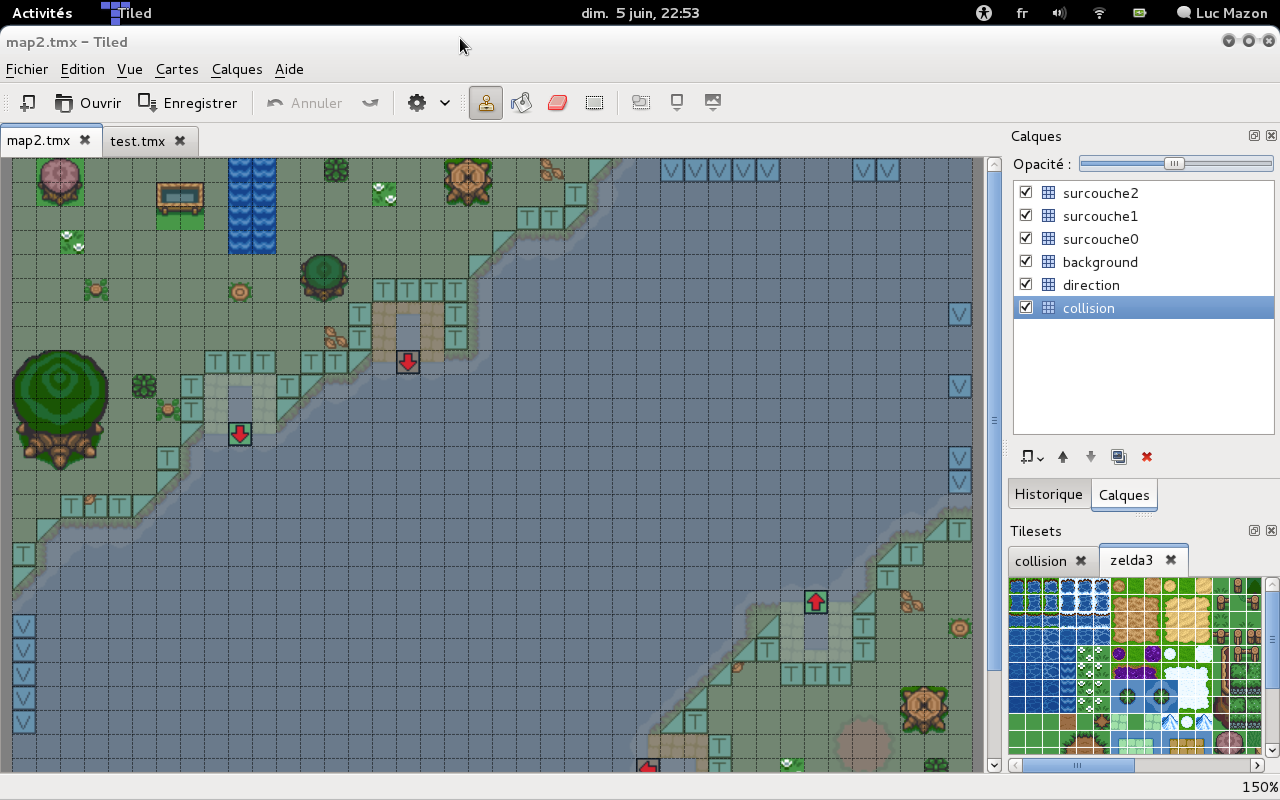
\includegraphics[width=0.8\textwidth]{images/tiled.png}
    \caption{Tiled Map Editor}
  \end{figure}
\end{frame}


\section{conclusion}
\begin{frame}[c]
  Avez-vous des questions ?
\end{frame}

\end{document}
